\documentclass[apj]{emulateapj}

\shorttitle{Fast Template Periodogram}
\shortauthors{Hoffman et al. 2016}

\usepackage[backref,breaklinks,colorlinks,citecolor=blue]{hyperref}
\usepackage[all]{hypcap}
%\renewcommand*{\backref}[1]{[#1]}
\usepackage{amsmath}


\newcommand{\todo}[1]{{\bf #1}}
\newcommand{\bigO}{\mathcal{O}}
\newcommand{\savg}[1]{\left<#1\right>}
\newcommand{\svar}{{\rm Var}}
\newcommand{\scov}{{\rm Cov}}
\newcommand{\Mshft}{\mathbf{M}_{\theta_2}}
\newcommand{\dMshft}{\partial\Mshft}
\newcommand{\dA}{\partial A}
\newcommand{\dB}{\partial B}

\newcommand{\hatyij}{\hat{y}^{(i)}_j}
\newcommand{\yij}{y^{(i)}_j}
\newcommand{\thta}[1]{\theta_{#1}^{(i)}}
\newcommand{\Mshftijsp}{\mathbf{M}_{\theta_2}^{(i)}}
\newcommand{\Mshftijmp}{\mathbf{M}_{\thta{2}}^{(i)}}
\newcommand{\Mshftkjsp}{\mathbf{M}_{\theta_2}^{(k)}}
\newcommand{\Mshftkjmp}{\mathbf{M}_{\thta{2}}^{(k)}}
\newcommand{\Mshfttld}{\widetilde{M}_{\theta_2}^{(i)}}
%\newcommand{\savg}[1]{\left<#1\right>}
\newcommand{\ybari}{\bar{y}^{(i)}}
\newcommand{\bandavg}[1]{\overline{#1}}
\newcommand{\MMhat}{\widehat{MM}}
\newcommand{\YMhat}{\widehat{YM}}
\newcommand{\Mbar}{\overline{M}}

\newcommand{\YCt}{\widetilde{YC}}
\newcommand{\YSt}{\widetilde{YS}}
\newcommand{\CCt}{\widetilde{CC}}
\newcommand{\CSt}{\widetilde{CS}}
\newcommand{\SSt}{\widetilde{SS}}





% read VERSION.txt for version
\newcommand{\versionfilename}{VERSION.txt}

\newwrite\versionfile

\AtBeginDocument{%
  \immediate\openin\versionfile=\versionfilename
  \read\versionfile to \versioninfo % \versioninfo is the macro containing the text line
\immediate\closein\versionfile% 
}
%%%%%%%%%%%%%%%%%%%%%%%%%%%%%%

\begin{document}

\title{A Fast Template Periodogram for Detecting Non-Sinusoidal Fixed-Shape Signals in Irregularly Sampled Time Series\\
         DRAFT VERSION \versioninfo }

\author{J. Hoffman\altaffilmark{1},
J. Vanderplas\altaffilmark{2},
J. Hartman\altaffilmark{1},
G. Bakos\altaffilmark{1}}
\email{jah5@princeton.edu}
%\email{jakevdp@cs.washington.edu}
%\email{jhartman@astro.princeton.edu}
%\email{gbakos@astro.princeton.edu}

\altaffiltext{1}{Department of Astrophysical Sciences, Princeton University, Princeton NJ 08540}
\altaffiltext{2}{eScience Institute, University of Washington, Seattle, WA 98195}

\begin{abstract}

    Astrophysical time series often contain periodic signals. The sheer volume of time series data from 
    photometric surveys demands computationally efficient methods for detecting and characterizing such signals. 
    The most efficient algorithms available for this purpose are those that exploit the 
    $\bigO(N\log N)$ scaling of the Fast Fourier Transform (FFT). However, these methods are not optimal 
    for non-sinusoidal signal shapes. Template fits (or periodic matched filters) optimize 
    sensitivity for \emph{a priori} known signal shapes but at enormous computational cost. Current 
    implementations of template periodograms scale as $\bigO(N_f N_{\rm obs})$, where $N_f$ is the number 
    of trial frequencies and $N_{\rm obs}$ is the number of lightcurve observations, and they do not 
    gaurantee the best fit at each trial frequency. In this work, we present a non-linear extension of the Lomb-Scargle 
    periodogram which provides a template-fitting algorithm that is both accurate (the exact optimal solutions are
    obtained except in rare cases) and computationally efficient (scaling as $\bigO(N_f\log N_f)$). 
    The non-linear optimization of the template fit at each frequency is recast as a polynomial 
    zero-finding problem, where the coefficients of the polynomial can be computed efficiently with
    FFTs. We show that our method, which uses truncated Fourier series to approximate templates, 
    is twice as fast as existing algorithms for small problems ($N\lesssim 10$ observations) and
    1-2 orders of magnitude faster for long base-line time series with $\bigO(10^4)$ observations.
    An open-source implementation of the fast template periodogram is available at 
    \href{https://www.github.com/PrincetonUniversity/FastTemplatePeriodogram}{github.com/PrincetonUniversity/FastTemplatePeriodogram}. 
\end{abstract}

\section{Introduction}\label{sec:introduction}

Astrophysical time series are challenging to analyze. Unlike
time series in other domains such as economics and finance, astrophysical 
observations are often irregularly sampled in time with heteroskedastic, 
non-Gaussian, and time-correlated measurement uncertainties.

Irregular sampling thwarts the straightforward application of many well-known 
time series tools like the discrete Fourier transform (DFT) and the auto-regressive 
moving average (ARMA) models. The DFT is a particularly unfortunate loss, since
the Fast Fourier Transform \citep{Cooley+Tukey_1965} reduces the $\bigO(N^2)$ DFT
to $\bigO(N\log N)$, and is a powerful tool for finding periodic signals.

The DFT can be extended to irregularly sampled data via what is sometimes
referred to as the classical periodogram \citep{Stoica+Li+He_2009}

\begin{equation}
    P_x(\omega) = \frac{1}{N^2}\left|\sum_{n=0}^{N - 1} y_n e^{- i \omega t_n}\right|^2.
\end{equation}

However, as \cite{Stoica+Li+He_2009} point out, this is not an
optimal measure of periodicity. A more robust estimate of the power spectrum is
given by the Lomb-Scargle periodogram \citep{Lomb_1976,Scargle_1982,Barning_1963,Vanicek_1971}.

ARMA models can also be extended to unevenly sampled data with the CARMA
model \citep{Kelly_etal_2014, Zinn_etal_2016}, but for the purposes of this paper, 
we focus solely on tools applicable to the detection of periodic signals in astrophysical data. 

The Lomb-Scargle periodogram and its extensions can be expressed in terms of 
least-squares minimization between the data $\{y_n\}_{n=1}^N$ and a model $\hat{y}$.
In the original formulation of the Lomb-Scargle periodogram, 

\begin{equation}
    \hat{y}_{\rm LS}(t|\theta, \omega) = \theta_0\cos{\omega t} + \theta_1\sin{\omega t}.
\end{equation}

This is equivalent to performing a DFT if the data is regularly sampled. The Lomb-Scargle
periodogram can be obtained from solving the linear system of equations that arise from
the condition that the summed squares of residuals between the data and the optimal
model,

\begin{equation}
\chi^2(\theta, S) \equiv \sum_i (y_i - \hat{y}(t_i|\theta) )^2,
\end{equation}

\noindent must be a local minimum. This means that

\begin{equation}
    \left.\frac{\partial\chi^2}{\partial\theta_i}\right|_{\theta=\theta_{\rm best}} = 0~~\forall\theta_i\in\theta.
\end{equation}

The resulting periodogram can be expressed as

\begin{equation}
\begin{split}
    P_{\rm LS} = \frac{1}{2\sigma^2}&\left(\frac{\left[\sum_{n=1}^N (y_n - \bar{y})\cos{\omega t_n}\right]^2}{\sum_{n=1}^N \cos^2{\omega t_i}} \right. \\
                &\left.+ \frac{\left[\sum_{n=1}^N (y_n - \bar{y})\sin{\omega t_n}\right]^2}{\sum_{n=1}^N \sin^2{\omega t_i}} \right),
\end{split}
\end{equation}

\noindent where $\bar{y} = \mathbb{E}[y_n]$, the mean of the data, and 
$\sigma = {\rm Var}(y_n)$, the variance of the data. 

Heteroskedasticity can be handled by using weighted least squares, 

\begin{equation}
\chi^2(\theta, S) \equiv \sum_i \frac{(y_i - \hat{y}(t_i|\theta) )^2}{\sigma_i^2},
\end{equation}

\noindent with weights $w_i = \frac{W}{\sigma_i^2}$, $W\equiv\sum \sigma_i^{-2}$ being
a normalization factor to ensure $\sum w_i = 1$, and correlated uncertainties
can be accounted for by using the full covariance matrix, $\Sigma_{ij} = {\rm Cov}\left((y_i - \bar{y})(y_j - \bar{y})\right)$.

\begin{equation}
\chi^2(\theta, S) \equiv (y_i - \hat{y}(t_i|\theta) )^{\rm T}\Sigma^{-1}(y_i - \hat{y}(t_i|\theta) ).
\end{equation}

If we assume the covariance matrix is diagonal, the Lomb-Scargle periodogram can be
evaluated quickly in one of two popular ways. The first, by \cite{Press+Rybicki_1989}
involves``extirpolating'' irregularly sampled data onto a regularly sampled mesh,
and then performing FFTs to evaluate the necessary sums. The second, as pointed
out in \cite{Leroy_2012}, is to use the non-equispaced FFT (NFFT) \cite{NFFT} to evaluate
the sums; this provides an order of magnitude speedup over the \cite{Press+Rybicki_1989}
algorithm, and both algorithms scale as $\bigO(N_f\log N_f)$.

There is a growing population of alternative methods for detecting
periodic signals in astrophysical data. Some of these methods can reliably
outperform the Lomb-Scargle periodogram, especially for non-sinusoidal signal shapes
(see \cite{Graham_etal_2013} for a recent empirical review of period finding algorithms). 
However, a key advantage the LS periodogram and its extensions is speed.
Virtually all other methods scale as $N_{\rm obs}\times N_f$, where $N_{\rm obs}$ is the number
of observations and $N_f$ is the number of trial frequencies, while the Lomb-Scargle
periodogram scales as $N_f\log N_f$. The virtual independence of Lomb-Scargle on the number
of observations (assuming $N_f \gtrsim N_{\rm obs}$) is especially attractive for lightcurves
with $N_{\rm obs} \gg \log N_f \sim 50$. 

Algorithmic efficiency will become increasingly important as the volume
of data produced by astronomical observatories continues to grow larger. The HATNet survey 
\citep{HATNet}, for example, has already made $\bigO(10^4)$ observations of 
$\bigO(10^6-10^7)$ stars. The Gaia telescope \citep{GAIA} is set to produce $\bigO(10-100)$ 
observations of $\bigO(10^9)$ stars. The Large Synoptic Survey Telescope (LSST; \cite{LSST}) 
will make $\bigO(10^2-10^3)$ observations of $\bigO(10^{10})$ stars during its operation starting in 2023.

This paper develops new extensions to least-squares spectral analysis for arbitrary
signal shapes. For non-periodic signals this method is known as matched filter analysis,
and can be extended to search for periodic signals by phase folding the data
at different trial periods. We refer to the latter technique, the subject of this paper, as
template fitting. 

Recently, \cite{Sesar_etal_2016} found that template fitting significantly improved
period and amplitude estimation for RR Lyrae in Pan-STARRS DR1 \citep{PanSTARRS}. Since the signal
shapes for RR Lyrae in various bandpasses are known \emph{a priori} (see \cite{Sesar_etal_2010}), 
template fitting provides an optimal estimate of amplitude and period,
given that the object is indeed an RR Lyrae star well modeled by at least one of the templates. 
Templates were especially crucial for Pan-STARRS data, since there are typically only 
35 observations per source over 5 bands \citep{Hernitschek_etal_2016}, not enough to obtain 
accurate amplitudes empirically by phase-folding. By including domain knowledge (i.e. knowledge of what RR Lyrae 
lightcurves look like), template fitting allows for accurate inferences of amplitude even 
for undersampled lightcurves.

However, the improved accuracy comes at substantial computational cost: the template fitting 
procedure took 30 minutes per CPU per object, and \cite{Sesar_etal_2016} were forced to limit
the number of fitted lightcurves ($\lesssim 1000$) in order to keep the computational costs
to a reasonable level. Several cuts were made before the template fitting step to reduce the
more than 1 million Pan-STARRS DR1 objects to a small enough number, and each of these steps
removes a small portion of RR Lyrae from the sample. Though this number was reported by
\cite{Sesar_etal_2016} to be small ($\lesssim 2\%$), it may be possible to further improve
the completeness of the final sample by applying template fits to a larger number of objects,
which would require either more computational resources, more time, or, ideally, a more efficient
template fitting procedure.

The paper is organized as follows. Section \ref{sec:derivations} poses the problem of template
fitting in the language of least squares spectral analysis and derives the fast template
periodogram. Section \ref{sec:implementation} describes a freely available implementation 
of the new template periodogram. Section \ref{sec:discussion} summarizes our results, 
addresses caveats, and discusses possible avenues for improving the efficiency of the current 
algorithm.


%Many astrophysical systems exhibit brightness fluctuations, and
%detecting these brightness fluctuations in data has been a challenge for astronomers for \todo{what was the
%earliest detection of variability?}. 

%Some of these variable systems, such as eclipsing binaries, transiting
%exoplanets, or pulsating stars, exhibit periodic brightness fluctuations. Powerful methods
%for detecting periodicities in observational data have been developed and deployed

%A plethora of astronomical systems exhibit periodic fluctuations
%in brightness. These systems are important for many reasons; pulsating
%stars are valuable laboratories for testing our understanding
%of stellar physics \todo{cite pulsating stars}, determining
%stellar composition \todo{cite astroseismology}, and as distance
%indicators \todo{cite distance indicators}. Transiting exoplanets
%are valuable 

\section{Derivations}\label{sec:derivations}

We define a template $\mathbf{M}$

\begin{equation}
    \mathbf{M} : [0, 1)\rightarrow\mathbb{R},
\end{equation}

\noindent as a mapping between the unit interval and the set of real numbers. We
restrict our discussion to sufficiently smooth templates such that
$\mathbf{M}$ can be adequately described by a truncated Fourier series

\begin{equation}
    \hat{\mathbf{M}}(\omega t|H) = \sum_{n=1}^H\left[c_n\cos{n\omega t} + s_n\sin{n\omega t}\right]
\end{equation}

\noindent for some $H > 0$. Specifically, we require that 

\begin{equation}
\begin{split}
   \forall t \in (0, 1]:\, \lim_{H\rightarrow\infty} \left|\mathbf{M}(t) - \hat{\mathbf{M}}(t|H)\right| = 0
\end{split}
\end{equation}

That the $c_n$ and $s_n$ values are \emph{fixed} (i.e., they define 
the template) is the crucial difference between the template periodogram and
the Multiharmonic Lomb Scargle (or FastChi) \citep{Palmer_2009}, where $c_n$ and $s_n$ 
are \emph{free parameters}.

We now construct a periodogram for this template. The periodogram assumes 
that an observed time series $S = \{(t_i, y_i, \sigma_i)\}_{i=1}^N$ can be modeled 
by a scaled, transposed template that repeats with period $2\pi / \omega$, i.e.

\begin{equation}
y_i \approx \hat{y}(\omega t_i|\theta, \mathbf{M}) = \theta_1\mathbf{M}(\omega t_i - \theta_2) + \theta_3,
\end{equation}

\noindent where $\theta\in \mathbb{R}^3$ is a set of model parameters. 

The optimal parameters are the location of a local minimum of the (weighted) sum of 
squared residuals,

\begin{equation}
    \chi^2(\theta, S) \equiv \sum_i w_i (y_i - \hat{y}(\omega t_i|\theta) )^2,
\end{equation}

\noindent and thus the following condition must hold for all three model parameters at 
the optimal solution $\theta=\theta_{\rm opt}$:

\begin{equation}\label{eq:chi2conds}
    \left.\frac{\partial\chi^2}{\partial\theta_j}\right|_{\theta=\theta_{\rm opt}} = 0~~\forall\theta_j\in\theta.
\end{equation}

Note that we have implicitly assumed $\chi^2(\theta,S)$ is a $C^1$ differentiable 
function of $\theta$, which requires that $\mathbf{M}$ is a
$C^1$ differentiable function. Though this assumption could be violated if we 
considered a more complete set of templates, (e.g. a box function), our restriction 
to truncated Fourier series ensures that $\mathbf{M}$ is
 $C^1$ differentiable and thus that $\chi^2(\theta,S)$ is $C^1$ differentiable.

Note that we also implicitly assume $\sigma_i > 0$ for all $i$ and we will later
assume that the variance of the observations $y_i$ is non-zero. If there are no
measurement errors, i.e. $\sigma_i = 0$ for all $i$, then uniform weights
(setting $\sigma_i = 1$) should be used. If the variance of the observations $y$ 
is zero, the periodogram is trivial and will be zero for all frequencies. We do not
consider the case where $\sigma_i = 0$ for some observations $i$ and $\sigma_j > 0$ for
some observations $j$. In that case, the weighted least squares estimator is undefined.

We can derive a system of equations for $\theta_{\rm opt}$ from the condition given 
in Equation \ref{eq:chi2conds}. The explicit condition that must be met for each parameter $\theta_j$ is simplified below,
using 

\begin{equation}
\hat{y}_i = \hat{y}(\omega t_i | \theta)
\end{equation}

\noindent and

\begin{equation}
\partial_j\hat{y}_i = \left.\frac{\partial \hat{y}(\omega t|\theta)}{\partial \theta_j}\right|_{t = t_i}
\end{equation}

\noindent for brevity:

\begin{equation}\label{eq:simpconds}
\begin{split}
0 &= \left.\frac{\partial\chi^2}{\partial\theta_j}\right|_{\theta=\theta_{\rm opt}}\\
  &= -2\sum_i w_i\left(y_i - \hat{y}_i \right)(\partial_j\hat{y})_i \\
\sum_i w_iy_i(\partial_j\hat{y})_i&= \sum_i w_i \hat{y}_i(\partial_j\hat{y})_i.
\end{split}
\end{equation}

The above is a general result that extends to all least squares periodograms.
To simplify derivations, we adopt the following notation:

\begin{eqnarray}
\savg{X} &\equiv& \sum_i w_i X_i\\
\savg{XY} &\equiv& \sum_i w_i X_iY_i\\
\scov(X, Y) &\equiv& \savg{XY} - \savg{X}\savg{Y}\\
\svar(X) &\equiv& \scov(X, X)
\end{eqnarray}

In addition, we denote the shifted template $\mathbf{M}(x - \theta_2)$ by $\Mshft(x)$.

For the amplitude and offset model parameters ($\theta_1$ and $\theta_3$, respectively), 
we obtain the following relations from Equation \ref{eq:simpconds}

\begin{eqnarray}
    \savg{y\Mshft(\omega t)} &=& \theta_1\savg{\Mshft^2(\omega t)} + \theta_3\savg{\Mshft(\omega t)}\\
    \label{eq:th3cond}
    \theta_3 &=& \bar{y} - \theta_1\savg{\Mshft(\omega t)},
\end{eqnarray}

\noindent where $\bar{y}\equiv \savg{y}$. Combining these expressions yields

\begin{equation}\label{eq:th13eq}
\theta_1 = \frac{\savg{(y - \bar{y})\Mshft(\omega t)}}{\svar(\Mshft(\omega t))}.
\end{equation}

For the offset parameter $\theta_2$, 

\begin{equation}
\label{eq:mshftdef1}
 \begin{split}
     \frac{\partial\hat{y}}{\partial\theta_2} &= \theta_1\frac{\dMshft}{\partial\theta_2}\\
     &= -\theta_1\dMshft,
 \end{split}
\end{equation}

\noindent where 

\begin{equation}
 \dMshft(x) = \sum_n \left[s_n\cos{n(x - \theta_2)} - c_n\sin{n(x - \theta_2)}\right].
\end{equation}
 
From Equations \ref{eq:simpconds}, \ref{eq:th3cond}, and \ref{eq:mshftdef1} we obtain

\begin{equation}\label{eq:th2eq}
 \theta_1 = \frac{\savg{(y - \bar{y})\dMshft(\omega t)}}{\scov\left(\Mshft(\omega t),\dMshft(\omega t)\right)},
\end{equation}

\noindent which, combined with Equation \ref{eq:th13eq}, provides 
a non-linear condition for $\theta_2$:

\begin{equation}\label{eq:th2cond}
\begin{split}
&\savg{(y - \bar{y})\dMshft(\omega t)}\svar(\Mshft(\omega t)) \\
 &= \savg{(y - \bar{y})\Mshft(\omega t)}\scov(\Mshft(\omega t),\dMshft(\omega t)).
\end{split}
\end{equation}

To obtain an explicit expression for Equation \ref{eq:th2cond},
we define several quantities, 

\begin{eqnarray}
CC_{nm} &\equiv& \scov(\cos{n\omega t},\cos{m\omega t})\label{eq:CCdef}\\
CS_{nm} &\equiv& \scov(\cos{n\omega t},\sin{m\omega t})\label{eq:CSdef}\\
SS_{nm} &\equiv& \scov(\sin{n\omega t},\sin{m\omega t})\label{eq:SSdef}\\
YC_n &\equiv& \savg{(y - \bar{y})\cos{n\omega t}}\label{eq:YCdef}\\
YS_n &\equiv& \savg{(y - \bar{y})\sin{n\omega t}}\label{eq:YSdef},
\end{eqnarray}

\noindent all of which can be evaluated quickly for every trial frequency 
$\omega$ with the use of NFFTs. We also obtain
an expression for the shifted template:

\begin{equation}
\begin{split}
    \Mshft(x) &= \sum_n \left[c_n\cos{n(x - \theta_2)} + s_n\sin{n(x - \theta_2)}\right]\\
    %\Mshft(x) &= \sum_n \left[c_n\left(\cos{nx}\cos{n\theta_2} + \sin{nx}\sin{n\theta_2}\right)\right. \\
    %        &\qquad\quad\left. + s_n\left(\sin{nx}\cos{n\theta_2} - \cos{nx}\sin{n\theta_2}\right)\right]\\
              &= \sum_n \left[\left(c_n\cos{n\theta_2} - s_n\sin{n\theta_2}\right)\cos{nx} \right.\\
              &\qquad\quad \left. + \left(s_n\cos{n\theta_2} + c_n\sin{n\theta_2}\right)\sin{nx}\right]\\
              &= \sum_n \left[\left(c_nT_n(u) \mp s_n\sqrt{1 - u^2}U_{n-1}(u)\right)\cos{nx} \right.\\
              &\qquad\quad \left. + \left(s_nT_n(u) \pm c_n\sqrt{1 - u^2}U_{n-1}(u)\right)\sin{nx}\right]\\
              &= \sum_n \left[A_n(u)\cos{nx} + B_n(u)\sin{nx}\right]
\end{split}
\end{equation}

\noindent where $u \equiv \cos \theta_2$, $T_n$ and $U_n$ are the Chebyshev polynomials 
of the first and second kind, respectively, and the $\pm$ ambiguity arises out of the
two possible signs for $\sin{\theta_2}$.

The derivatives of first and second order Chebyshev polynomials are known to be

\begin{eqnarray}
\frac{dT_n}{dx} &=& nU_{n-1}(x)\\
\frac{dU_n}{dx} &=& \frac{(n+1)T_{n+1}(x) - xU_n(x)}{x^2 - 1},
\end{eqnarray}

\noindent and this implies that the first derivative of the shifted template is

\begin{equation}
\begin{split}
\dMshft(x) &= \sum_n \left[n\left(c_nU_{n-1}(u) \pm s_n\frac{T_n(u)}{\sqrt{1 - u^2}}\right)\cos{nx} \right.\\
           &\qquad\quad \left. + n\left(s_nU_{n-1}(u) \mp c_n\frac{T_n(u)}{\sqrt{1 - u^2}}\right)\sin{nx}\right]\\
\dMshft(x) &= \sum_n \left[\dA_n(u) \cos{nx} + \dB_n(u) \sin{nx}\right]
\end{split}
\end{equation}

Using the sums provided in Equations \ref{eq:CCdef} -- \ref{eq:YSdef}, writing 
$A_n$ and $B_n$ as as shorthand for $A_n(u)$ and $B_n(u)$, and employing 
Einstein summation notation, we have that

\begin{align}
\savg{(y - \bar{y})\Mshft} &= A_n YC^n + B_n YS^n\\
\savg{(y - \bar{y})\dMshft} &= \dA_n YC^n + \dB_n YS^n\\
\svar(\Mshft) &= 
\begin{aligned}[t]
&A_nA_m CC^{nm} \\
& + 2A_nB_m CS^{nm}
+ B_nB_m SS^{nm}
\end{aligned}\\
\scov(\Mshft, \dMshft) &=
\begin{aligned}[t]
&A_n \dA_m CC^{nm}\\
&+ (A_n\dB_m + B_n \dA_m)CS^{nm} \\
&+ B_n\dB_m SS^{nm}
\end{aligned}.
\end{align}

Equation \ref{eq:th2cond} now becomes

%\begin{widetext}
\begin{align}\label{eq:polynomial}
0 &= 
\begin{aligned}[t]
&\quad A_nA_m\dA_k\left(YC^nCC^{mk} -  YC^kCC^{mn}\right)\\
&+ A_nA_m\dB_k\left(YC^nCS^{mk} - YS^kCC^{mn}\right)\\
&+ A_nB_m\dA_k\left(YC^nCS^{km} + YS^mCC^{kn}\right)\\
&+ A_nB_m\dB_k\left(YC^nSS^{mk} + YS^mCS^{nk}\right)\\
&+ B_nB_m\dA_k\left(YS^nCS^{km} - YC^kSS^{nm}\right)\\
&+ B_nB_m\dB_k\left(YS^nSS^{mk} - YS^kSS^{mn}\right).
\end{aligned}
\end{align}
%\end{widetext}

Each $AA\dA$, $AA\dB$, ..., $BB\dB$ can be expressed as 

\begin{equation}
AA\dA,~AA\dB,~...= p(u) + (1 - u^2)^{-1/2}q(u),
\end{equation}

\noindent where both $p(u)$ and $q(u)$ are polynomials in $u$. Therefore, Equation
\ref{eq:polynomial} can be expressed in the same form, and if we assume $|u| < 1$,
a polynomial condition can be obtained

\begin{equation}\label{eq:polycond}
0 = (1 - u^2)\hat{p}^2(u) - \hat{q}^2(u) = \hat{P}(u)\quad |u| < 1
\end{equation}

\noindent for some polynomials $\hat{p}, \hat{q}$, and $\hat{P}$.

Here and in the implementation presented in Section \ref{sec:implementation}, we
do not attempt to obtain an explicit form for the polynomials $\hat{p},\,\,\hat{q},\,\,\hat{P},\,\,...$.
We compute these polynomials as needed with polynomial algebra and the relation given 
in Equation \ref{eq:polynomial}, and precompute the polynomials $AA\dA,\,\,AA\dB,\,\,...$ 
for each template, since they do not depend on the data. 

We solve for the zeros of the polynomial condition defined by Equation \ref{eq:polycond}
using the \texttt{numpy.polynomial.polyroots} function, which solves for the eigenvalues 
of the polynomial companion matrix. We also test the special cases where $u=1$, 
i.e. $\theta_2 \in \{ 0, \pi \}$. 

The set of real roots of $\hat{P}$, $R\in \mathcal{R}$, provides a set of $\theta_2$ parameters,
one of which is the optimal value. We evaluate the periodogram at each $\theta_2 \in R\cup\{-1,1\}$
to find the optimal value of $\theta_2$.

%%%%%%%%%%%%%%%%%%%%%%% TODO: FINISH

An explicit form of the polynomial given in Equation \ref{eq:polynomial} may provide some
shortcuts that could further improve computational efficiency. As discussed in Section
\ref{sec:compreqs} and \ref{sec:implementation}, deriving the polynomial $\hat{P}$ and finding
its real roots is the limiting computational step for the FTP. The efficiency of the root finding step
is aided by the fact that $\hat{P}$ is a polynomial, and thus the roots can be approximated 
by the eigenvalues of the polynomial companion matrix, or by a variety of other methods \todo{cite rootfinding
methods}, which in many cases are faster and more accurate than general non-linear root finding methods
\todo{this should be backed up more.}

We have derived an explicit, non-linear system of equations to solve for
the parameters $\theta_1$, $\theta_2$, and $\theta_3$. Solving this system of equations
requires finding the zeros of a polynomial $\hat{P}(u)$ at the given trial frequency.


\subsection{Negative amplitude solutions}
The model $\hat{y}= \theta_1\Mshft + \theta_0$ allows for $\theta_1 < 0$ solutions. 
In the original formulation of Lomb-Scargle and in linear
extensions involving multlple harmonics, negative amplitudes translate to
phase differences, since $-\cos{x} = \cos(x - \pi)$ and $-\sin{x} = \sin(x - \pi)$.

However, for non-sinusoidal templates, $\mathbf{M}$, negative amplitudes
do not generally correspond to a phase difference. For example, a 
detached eclipsing binary template $\mathbf{M}_{\rm EB}(x)$ cannot be 
expressed in terms of a phase-shifted negative eclipsing binary template; i.e.
$\mathbf{M}_{\rm EB} \neq - \mathbf{M}_{\rm EB}(x - \phi)$ for any $\phi\in[0, 2\pi)$.

Negative amplitude solutions found by the fast template periodogram are usually
undesirable, as they may produce false positives for lightcurves that resemble
flipped versions of the desired template, and allowing for $\theta_1 < 0$ solutions
increases the number of effective free parameters of the model, which lowers
the signal to noise, especially for weak signals.

One possible remedy for this problem is to set $P_{\rm FTP}(\omega) = 0$ if the optimal
solution for $\theta_1$ is negative, but this complicates the interpretation of $P_{\rm FTP}$.
Another possible remedy is, for frequencies that have a $\theta_1 < 0$ solution, 
to search for the optimal parameters while enforcing that $\theta_1 > 0$,
e.g. via non-linear optimization, but this likely will eliminate the computational
advantage of FTP over existing methods.

Thus, we allow for negative amplitude solutions in the model fit and caution
the user to check that the best fit $\theta_1$ is positive. Negative amplitude
solutions may only be a problem for weak signals, or signals that, when flipped, 
are similar to other astrophysical signals.


\subsection{Extending to multi-band observations}

\subsubsection{Multi-phase model}
\label{sec:multiband}
As shown in \cite{Vanderplas+Ivezic_2015}, the multi-phase periodogram (their 
$(N_{\rm base}, N_{\rm band}) = (0, 1)$ periodogram), for any model can
be expressed as a linear combination of single-band periodograms:

\begin{equation}
\label{eq:multibandmultiphase}
P^{(0,1)}(\omega) = \frac{\sum_{k=1}^K\chi^2_{0, k}P_{k}(\omega)}{\sum_{k=1}^K\chi^2_{0,k}}
\end{equation} 

\noindent where $K$ denotes the number of bands, $\chi^2_{0,k}$ is the weighted sum of squared
residuals between the data in the $k$-th band and its weighted mean $\savg{y}$, and $P_k(\omega)$ is
the periodogram value of the $k$-th band at the trial frequency $\omega$. 

With Equation \ref{eq:multibandmultiphase}, the template periodogram is readily applicable to multi-band 
time series, which is crucial for experiments like LSST, SDSS, Pan-STARRS, and other current 
and future photometric surveys.

\subsubsection{Shared-phase model}
Extending the template periodogram to multi-band observations while fixing the
relative phases of the templates requires additional derivation. A shared-phase
model has $2K + 1$ free parameters, with an offset and amplitude for each filter 
and a shared phase term.

The $\chi^2$ corresponding to the shared-phase multiband model is

\begin{equation}
\label{eq:chi2sharedphase}
\chi^2 = \sum_i^K\sum_j^{N_i} w_j^{(i)}(\yij - \hatyij)^2,
\end{equation}

\noindent where $\hatyij = \thta{1}\Mshftijsp + \thta{3}$ represents the model corresponding to a given
filter $i$. The system of equations derived by setting $\partial_\theta \chi^2 = 0$ for each parameter $\theta$
reduces to the familiar expressions for the amplitude and offset:

\begin{eqnarray}
\thta{1} &=& \frac{\savg{(\yij-\ybari)\Mshftijsp}}{\svar(\Mshftijsp)}\\
\thta{3} &=& \ybari - \thta{1}\svar(\Mshftijsp),
\end{eqnarray}

as well as a non-linear relation that must be satisfied for the shared-phase
parameter:
\begin{widetext}
\begin{align}
\label{eq:condsharedphase}
\sum_i^M\savg{(\yij-\ybari)\Mshftijsp}&\left(\prod_{k\ne i}\left(\svar\left(\Mshftkjsp\right)\right)^2\right)\\
&\times \left(\savg{(\yij-\ybari)\partial\Mshftijsp}\svar\left(\Mshftijsp\right) - \savg{(\yij-\ybari)\Mshftijsp}\scov\left(\Mshftijsp,\partial\Mshftijsp\right)\right) = 0.
\end{align}
\end{widetext}


\subsubsection{Other multi-band extensions}
Other multi-band template periodograms are derivable; for instance, \cite{Sesar_etal_2016} used what amounted
to a shared phase, amplitude, and offset model. Their model can be translated to

\begin{equation}
\hatyij = \theta_1\left(\underbrace{\alpha^{(i)}\Mshftijsp + \beta^{(i)}}_{\widetilde{M}_{\theta_2}^{(i)}}\right) + \theta_3
\end{equation}

where the $\alpha^{(i)}$ and $\beta^{(i)}$ parameters are fixed. This model has only 3 free parameters,
which allowed \cite{Sesar_etal_2016} to achieve high signal-to-noise despite having less than
10 epochs in each band. 

In this case, the requirement that $\partial_{\theta_1}\chi^2 = 0$ gives

\begin{align}
0 &= \sum_i^K \savg{\yij\Mshfttld} - \theta_1\sum_i^K\savg{\left(\Mshfttld\right)^2}\\
&\quad\quad - \theta_3\sum_i^K\savg{\Mshfttld}.
\end{align}

Requiring $\partial_{\theta_3}\chi^2 = 0$ gives another relation between
the offset and amplitude parameters

\begin{align}
0 &= \sum_i^K\ybari - \theta_1\sum_i^K\savg{\Mshfttld} - K\theta_3\\
\implies \theta_3 &= \bandavg{\ybari} - \theta_1\bandavg{\savg{\Mshfttld}}.
\end{align}

which implies that

\begin{align}
0 &= \sum_i^K \savg{\yij\Mshfttld} - \theta_1\sum_i^K\savg{\left(\Mshfttld\right)^2} \\
  &\quad\quad - K\bandavg{\ybari}\bandavg{\savg{\Mshfttld}} + K\theta_1\bandavg{\savg{\Mshfttld}}^2\\
  &= \bandavg{\savg{(\yij - \bandavg{\ybari})\Mshfttld}} - \theta_1\left(\bandavg{\savg{\left(\Mshfttld\right)^2}}\right. \\
  &\quad\quad \left. - \bandavg{\savg{\Mshfttld}}^2\right)\\
\theta_1 &= \frac{\bandavg{\savg{(\yij - \bandavg{\ybari})\Mshfttld}}}{\bandavg{\savg{\left(\Mshfttld\right)^2}} - \bandavg{\savg{\Mshfttld}}^2}
\end{align}


Where here, $\bandavg{\cdot}$ denotes a quantity averaged over all bandpasses.
Combining these relations with the requirement that $\partial_{\theta_2}\chi^2 = 0$, i.e.

\begin{align}
0 &= \theta_1 \sum_i^M\savg{\yij\partial\Mshfttld} - \theta_1\savg{\Mshfttld\partial\Mshfttld} \\
  &\quad\quad - \theta_3\savg{\partial\Mshfttld},
\end{align}

produces the condition that must be satisfied by the optimal phase parameter $\theta_2$,

\begin{widetext}
\begin{equation}
\bandavg{\savg{(\yij - \bandavg{\ybari})\partial\Mshfttld}}\left(\bandavg{\savg{\left(\Mshfttld\right)^2}} - \bandavg{\savg{\Mshfttld}}^2\right)
- \bandavg{\savg{(\yij - \bandavg{\ybari})\Mshfttld}}\left(\bandavg{\savg{\Mshfttld\partial\Mshfttld}} 
- \bandavg{\savg{\Mshfttld}}\bandavg{\savg{\partial\Mshfttld}}\right).
\end{equation}
\end{widetext}


\subsection{Computational requirements}\label{sec:compreqs}

For a given number of harmonics $H$, the task of deriving 
$\hat{P}$ requires a triple sum over $H$ terms, with each sum
requiring $\bigO(n_{\hat{P}})$ operations, where $n_{\hat{P}}$ is the order
of $\hat{P}$. The order of $\hat{P}$ can be shown to be

\begin{equation}
6H - {\rm deg}\left({\rm gcf}\left((1 - u^2)\star\hat{p}^2, \hat{q}^2\right)\right) \propto H,
\end{equation}

\noindent where ${\rm gcf}(p_1, p_2)$ denotes the greatest common polynomial factor
between polynomials $p_1$ and $p_2$, and ${\rm deg}(p)$ denotes the degree of polynomial $p$. 
Computing the coefficients of $\hat{P}$ therefore scales as $\bigO(H^4)$ at each trial frequency. 

The computational complexity of polynomial root finding
is algorithm dependent. If we choose to perform singular value decomposition of
the polynomial companion matrix\footnote{The \texttt{numpy.polynomial.polyroots} 
function uses this method.}, the root finding step scales as 
$\bigO(n_{\hat{P}}^3) = \bigO(H^3)$. The polynomial root-finding step 
should be asymptotically faster (for large $H$) than the computation of 
the polynomial coefficients.

When considering $N_f$ trial frequencies, the polynomial computation and root-finding 
step scales as $\bigO(H^4N_f)$. The computation of the sums 
(Equations \ref{eq:CCdef} -- \ref{eq:YSdef}) scales as $\bigO(HN_f\log HN_f)$.
Therefore, the entire template periodogram scales as 

\begin{equation}
\bigO(HN_f \log HN_f + H^4N_f).
\end{equation}

\begin{figure}
    \centering
    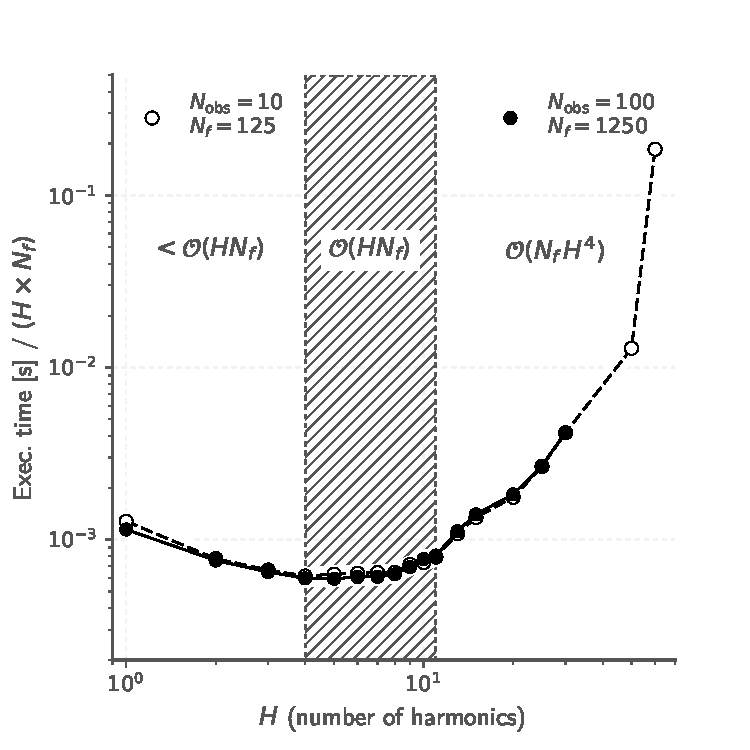
\includegraphics[width=0.5\textwidth]{plots/timing_vs_nharm.pdf}
    \caption{\label{fig:timingnharm} Computation time of FTP scaled by $NH$ for
            different numbers of harmonics. For $H\lesssim 3$, FTP scales
            sublinearly in $H$ (possibly due to a constant overhead per
            trial frequency, independent of $H$). When $3 \lesssim H \lesssim 11$,
            FTP scales approximately linearly in $H$, and when $H \gtrsim 11$
            FTP approaches the $\bigO(H^4)$ scaling limit.}
\end{figure}

For a fixed number of harmonics $H$, the template periodogram scales as
$\bigO(N_f\log N_f)$. However, for a constant number of trial frequencies $N_f$, 
the template algorithm scales as $\bigO(H^4)$, and computational resources
alone limit $H$ to reasonably small numbers $H\lesssim15$ (see Figure \ref{fig:timingnharm}).


\subsubsection{Computational considerations of multi-band extensions}
Multi-band extensions generally require more computational
time than the single band case. For the shared-phase multi-band periodogram,
the scaling becomes $\bigO{KHN_f\log HN_f + K^4H^4N_f}$. The final expression given
in Equation \ref{eq:condsharedphase} produces a root-finding polynomial that is of order
$2H(5K - 1)$ for $K > 1$, compared with the order $\sim 6H$ polynomial obtained for
the $K=1$ case.

For the shared phase, amplitude, and offset case, however, the polynomial
order remains the same as for the single band case, though the time needed to compute
the polynomial coefficients increases by a factor of $K$. 

\section{Implementation}\label{sec:implementation}

\begin{figure*}
    \centering
    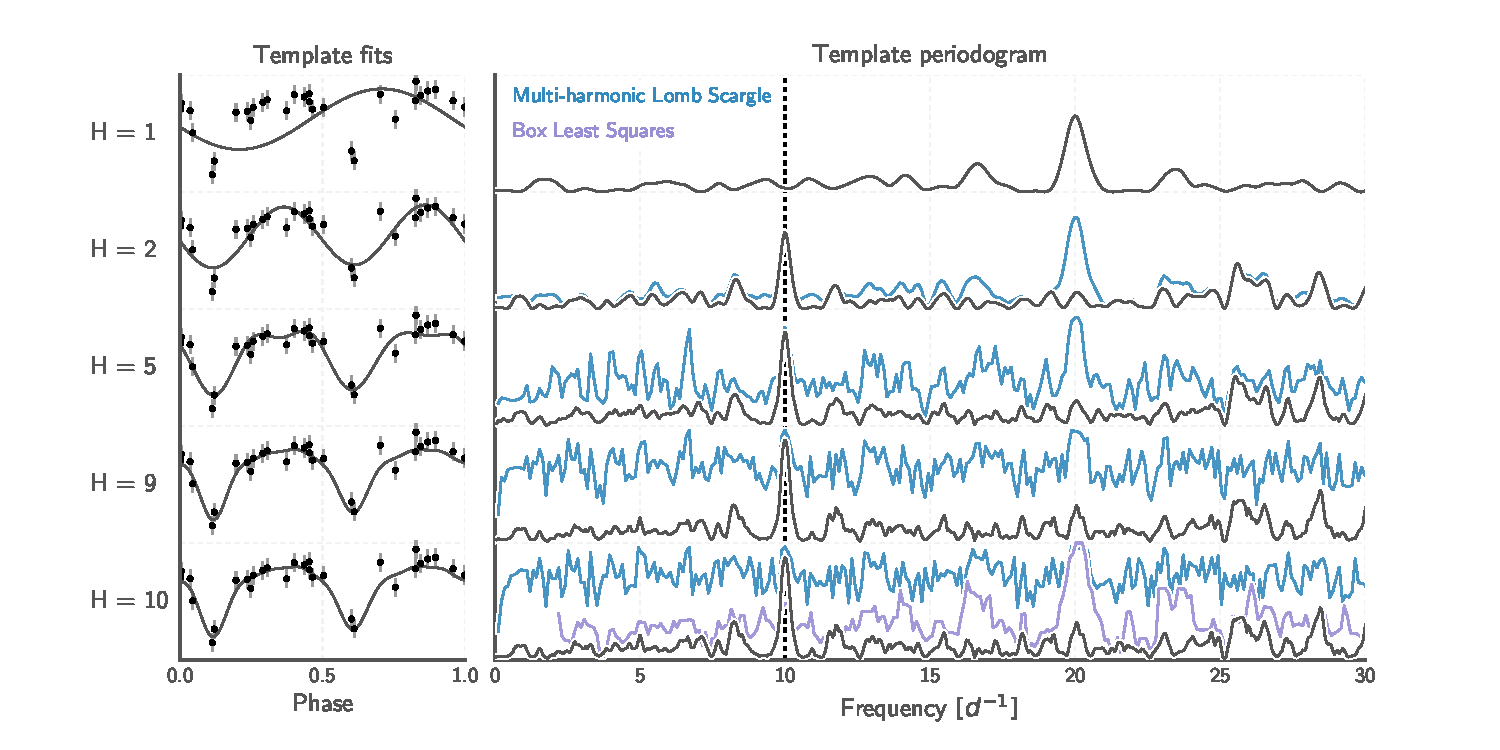
\includegraphics[width=\textwidth]{plots/templates_and_periodograms.pdf}
    \caption{\label{fig:tempsandpdgs} Template periodograms performed on a simulated eclipsing
            binary lightcurve (shown phase-folded in the left-hand plots). The top-most plot 
            uses only one harmonic, equivalent to a Lomb-Scargle periodogram. Subsequent plots
            use an increasing number of harmonics, which produces a narrower and higher peak
            height around the correct frequency. For comparison, the multi-harmonic extension 
            to Lomb-Scargle is plotted in blue, using the same number of harmonics as the FTP.
            The Box Least-Squares \citep{Kovacs_2002} periodogram is shown in the final plot.}
\end{figure*}

An open-source implementation of the template periodogram in Python is
available.\footnote{\url{https://github.com/PrincetonUniversity/FastTemplatePeriodogram}} 
Computing $\hat{P}(u)$ is done using the \texttt{numpy.polynomial} module 
\citep{Scipy}. The \texttt{nfft} Python module,
\footnote{https://github.com/jakevdp/nfft} which provides a Python 
implementation of the non-equispaced fast Fourier transform \citep{NFFT}, 
is used to compute the necessary sums for a particular time series.

No explicit parallelism is used anywhere in the current implementation, 
however certain linear algebra operations in \texttt{Scipy} use OpenMP 
via calls to BLAS libraries that have OpenMP enabled.

All timing tests were run on a quad-core 2.6 GHz Intel Core i7 MacBook 
Pro laptop (mid-2012 model) with 8GB of 1600 MHz DDR3 memory. The \texttt{Scipy} stack 
(version 0.18.1) was compiled with multi-threaded MKL libraries.
However, the slowest portion of the algorithm, computing the polynomial
coefficients, uses the \texttt{numpy.einsum} function which is not
multi-threaded. 

\subsection{Comparison with non-linear optimization}

Within the Python implementation of the FTP, we have provided access to slower 
methods that employ non-linear optimizationto compare the accuracy and speed 
of the template periodogram described in this paper.

Periodograms computed in Figures \ref{fig:tempsandpdgs}, \ref{fig:corrwgats},
and \ref{fig:corrwhighh} used simulated data. The simulated data has uniformly
random observation times, with gaussian-random, homoskedastic, uncorrelated 
uncertainties. An eclipsing binary template, generated by fitting a well-sampled,
high signal-to-noise eclipsing binary in the HATNet dataset (BD+56 603)
with a 10-harmonic truncated Fourier series.

\subsubsection{Accuracy}

\begin{figure}
    \centering
    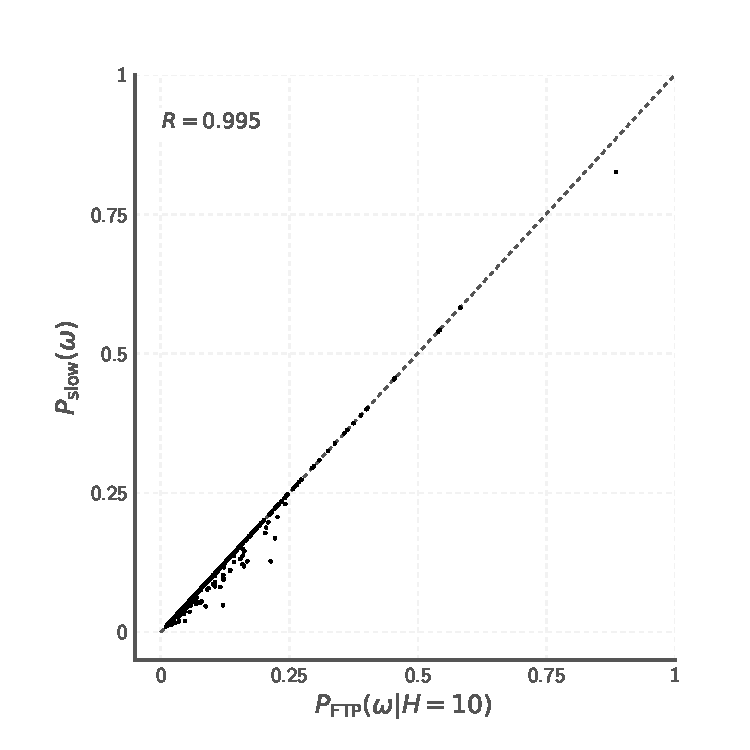
\includegraphics[width=0.5\textwidth]{plots/correlation_with_nonlinopt.pdf}
    \caption{\label{fig:corrwgats} Comparing accuracy between previous methods that rely
            on non-linear optimization at each trial frequency with the fast template periodogram 
            described in this paper. Both methods are applied to the same simulated data as shown 
            in Figure \ref{fig:tempsandpdgs}.
            The FTP consistently finds more optimal template fits than 
            those found with non-linear optimization, which do not gaurantee convergence to 
            a globally optimal solution. The FTP solves for the optimal
            fit parameters directly, and therefore is able to achieve greater accuracy than template
            fits done via non-linear optimization.}
\end{figure}

\begin{figure*}
    \centering
    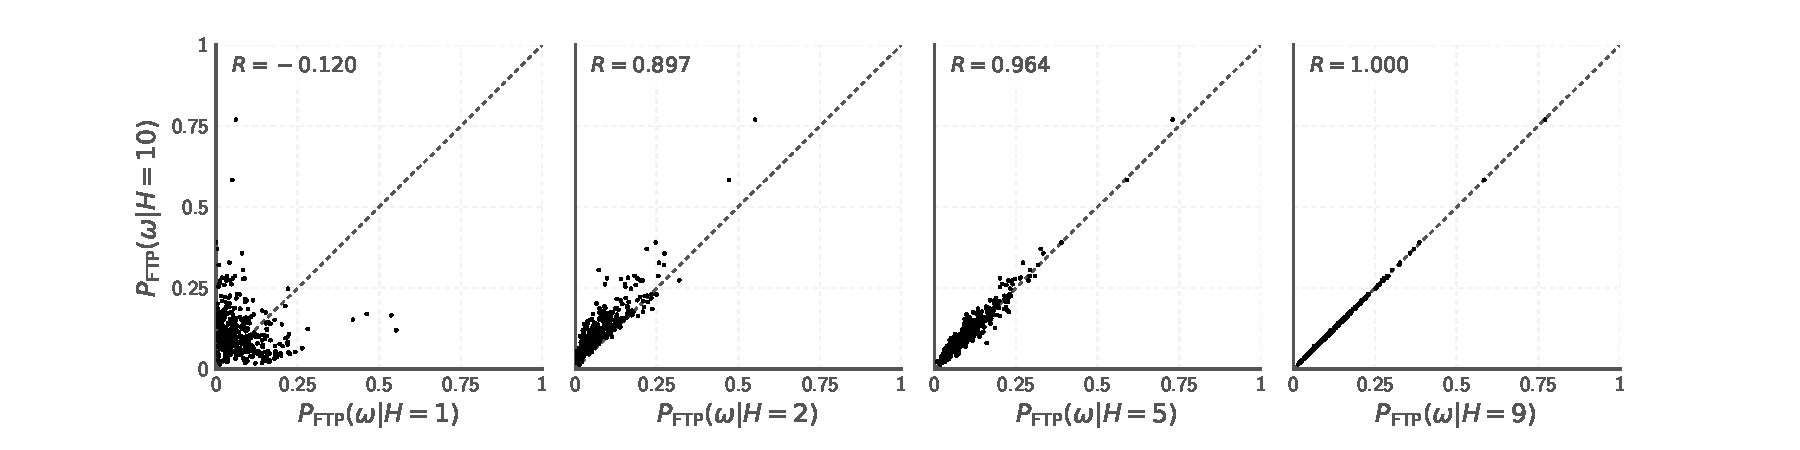
\includegraphics[width=\textwidth]{plots/correlation_with_large_H.pdf}
    \caption{\label{fig:corrwhighh} Comparing the template periodogram calculated with $H=10$ harmonics
            to the template periodogram using a smaller number of harmonics $H < 10$. The template and
            data used to perform the periodogram calculations are the same as those shown in Figure \ref{fig:tempsandpdgs}.}    
\end{figure*}

For weak signals or signals folded at the incorrect trial period, there
may be a large number of local $\chi^2$ minima in the parameter space, and thus
non-linear optimization algorithms may have trouble finding the global minimum. The 
FTP, on the other hand, solves for the optimal parameters directly, and
thus is able to recover optimal solutions even when the signal is weak
or not present.

Figure \ref{fig:corrwgats} illustrates the accuracy improvement with FTP.
Many solutions found via non-linear optimization are significantly suboptimal
compared to the solutions found by the FTP.

Figure \ref{fig:corrwhighh} compares FTP results obtained using the full template
$(H=10)$ with those obtained using smaller numbers of harmonics. The left-most
plot compares the $H=1$ case (weighted Lomb-Scargle), which, as also demonstrated
in Figure \ref{fig:tempsandpdgs}, illustrates the advantage of the template
periodogram for known, non-sinusoidal signal shapes.


\subsubsection{Computation time}

\begin{figure*}
    \centering
    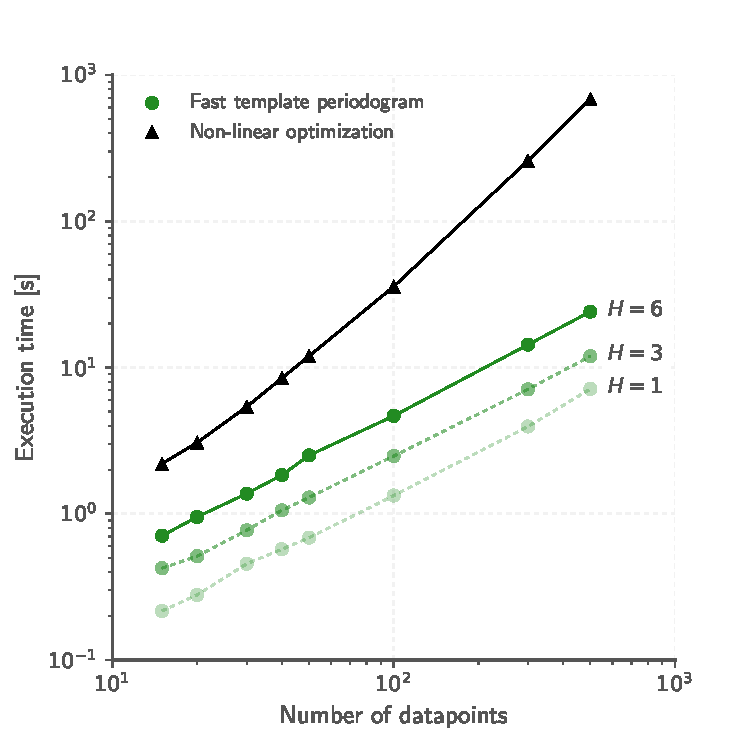
\includegraphics[width=0.45\textwidth]{plots/timing_vs_ndata.pdf}
    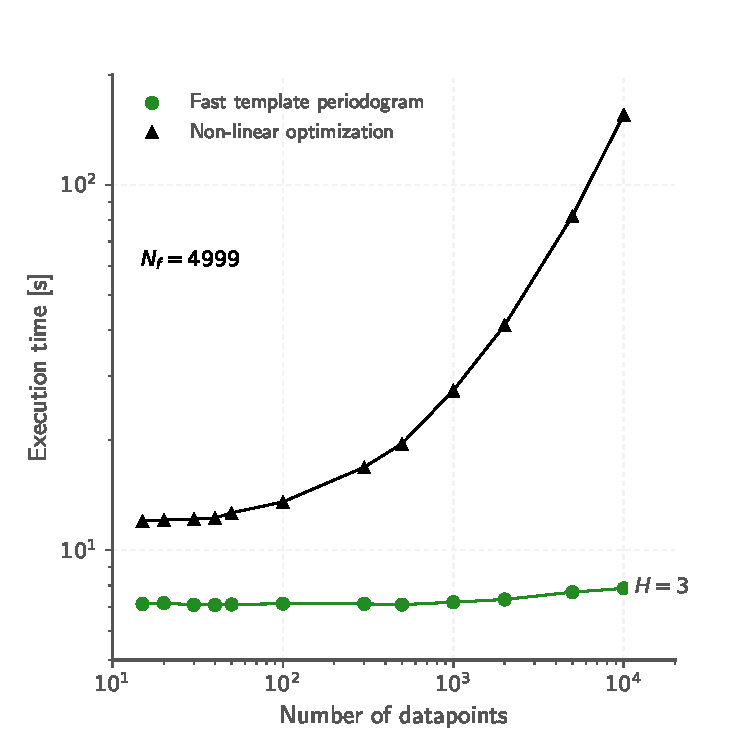
\includegraphics[width=0.45\textwidth]{plots/timing_vs_ndata_const_freq.pdf}
    \caption{\label{fig:timingndata} Computation time of FTP compared with alternative techniques
             that use non-linear optimization at each trial frequency. \emph{Left}: timing for the
             case when $N_f = ~12 N_{\rm obs}$, i.e. the cadence of the observations is constant. 
             \emph{Right}: timing for the case when $N_f$ is fixed, i.e. the baseline of the observations
             are constant. Non-linear optimization techniques scale as $\bigO(N_f N_{\rm obs})$ while 
             the FTP scales as $\bigO(HN_f\log HN_f + N_fH^4)$, where $H$ is the number of harmonics
             needed to approximate the template.}
    
\end{figure*}

FTP scales asymptotically as $\bigO(N_fH\log N_fH)$ with respect to the number of trial frequencies,
$N_f$ and as $\bigO(N_fH^4)$ with respect to the number of harmonics in which the template is expanded, $H$.
However, for reasonable cases ($N_f \lesssim 10^{120}$ when $H=5$) the computation time is dominated by
computing polynomial coefficients and root finding, both of which scale linearly in $N_f$. 

The number of trial frequencies needed for finding astrophysical signals in a typical photometric time series is

\begin{equation}
N_f = 1.75 \times 10^6 \left(\frac{{\rm baseline}}{10~{\rm yrs}}\right)\left(\frac{\alpha}{5}\right)\left(\frac{15~{\rm mins}}{P_{\rm min}}\right)
\end{equation}

\noindent where $\alpha$ represents the ``oversampling factor,'' $\Delta f_{\rm peak} / \Delta f$, where $\Delta f_{\rm peak} \sim 1/{\rm baseline}$ is
the typical width of a peak in the periodogram and $\Delta f$ is the frequency spacing of the periodogram.

Extrapolating from the timing of a test case (500 observations, 5 harmonics, 15,000 trial frequencies), the summations
account for approximately 5\% of the computation time when $N_f \sim 10^6$. If polynomial computations and
root-finding can be improved to the point where they no longer dominate the computation time, this would provide an
order of magnitude speedup over the current implementation.

Figure \ref{fig:timingndata} compares the timing of the FTP with that of previous methods that employ
non-linear optimization. For the case when $N_f\propto N_{\rm obs}$, FTP achieves a factor of 3 speedup for even 
the smallest test case (15 datapoints), while for larger cases ($N\sim10^4$) FTP offers 2-3 orders of magnitude 
speed improvement. For the constant baseline case, FTP is a factor of $\sim 2$ faster for the smallest test case
and a factor of $\sim 20$ faster for $N_{\rm obs}\sim 10^4$. Future improvements to the FTP implementation
could further improve speedups by 1-2 orders of magnitude over non-linear optimization.


% The 10^120 figure comes from the fact that for a test case (Ndata = 500, H = 5, Nf = 14917), 
% The fast summations take 8.905e-05 s / freq and the autopower() method takes 2.561e-03 s / freq.
% The fast summation step scales as Nf \log Nf while the rest of the steps scale as Nf (for constant H)
% So we have that 
%    t_sums/freq  = alpha * log10(Nf)
%    t_other/freq = beta 
%
% t_total(Nf0) = 2.561e-03 = t_sums(Nf0) + t_other(Nf0) = alpha * log10(Nf0) + beta
% and t_sums(Nf0) = 8.905e-05 = alpha * log10(Nf0)
% so alpha = 8.905e-05 / (log10(14917)) = 2.134e-05
% and beta = (2.64E-3 - 8.905e-05) = 2.55e-3
% beta/alpha = 120

% f_sums = t_sums(Nf) / t_total(Nf) = alpha * log10(Nf) / (beta + alpha * log10(Nf))
% f_sums ( beta + alpha log10(Nf)) = alpha * log10(Nf)
% alpha * ( 1 - f_sums) * log10(Nf) = f_sums * beta
% log10(Nf) = (beta / alpha) * (f_sums / (1 - f_sums))
% Nf = 10 ^ ((beta / alpha) * (f_sums / (1 - f_sums)))
% 
% Nf = 10 ^ (120 * (f_sums / (1 - f_sums)))
% when f_sums = 0.5 (the point at which the summations dominate the computation time)
% Nf = 10^120!!

 

\section{Discussion}\label{sec:discussion}

Template fitting is a powerful technique for accurately recovering
the period and amplitude of objects with \emph{a priori} known
lightcurve shapes. It has been used in the literature by, e.g.
\cite{Sesar_etal_2016, Sesar_etal_2010}, to analyze RR Lyrae in the
SDSS and PS1 datasets, where it has been shown to produce purer
samples of RR Lyrae at a given completeness. The computational
cost of current template fitting algorithms, however, limits their
application to larger datasets or with a larger number of templates.

We have presented a novel template fitting algorithm that extends
the Lomb-Scargle periodogram \citep{Lomb_1976,Scargle_1982,Barning_1963,Vanicek_1971}
to handle non-sinusoidal signals that can be expressed in terms of
a truncated Fourier series with a reasonably small number of harmonics
($H\lesssim 10$). 

The fast template periodogram (FTP) asymptotically scales as 
$\bigO(N_fH\log N_fH + N_fH^4)$, while previous template fitting algorithms
such as the one used in the \texttt{gatspy} library \citep{gatspy},
scale as $\bigO(N_fN_{\rm obs})$. However, the FTP effectively
scales as $\bigO(N_fH^4)$, since the time needed to compute polynomial
coefficients and perform zero-finding dominates the computational time
for all practical cases ($N_f \lesssim 10^{120}$).
The $H^4$ scaling effectively restricts templates to those that are
sufficiently smooth to be explained by a small number of Fourier terms.

FTP also improves the accuracy of previous template fitting algorithms, 
which rely on non-linear optimization at each trial frequency to minimize
the $\chi^2$ of the template fit. The FTP routinely finds superior fits over
non-linear optimization methods.

An open-source Python implementation of the FTP is available at
GitHub.\footnote{\url{https://github.com/PrincetonUniversity/FastTemplatePeriodogram}} 
The current implementation could likely be improved by:

\begin{enumerate}
    \item Improving the speed of the polynomial
          coefficient calculations and the zero-finding steps. This could potentially yield
          a speedup of $\sim1-2$ orders of magnitude over the current implementation.
    \item Exploiting the embarassingly parallel nature of the FTP using GPU's.
\end{enumerate}

For a constant baseline, the current implementation improves existing methods by factors 
of a $\sim$few for lightcurves with $\bigO(100)$ observations, and by an order of magnitude 
or more for objects with more than 1,000 observations. These improvements, taken at face
value, are not enough to make template fitting feasible on LSST-sized datasets. However,
optimizing the polynomial computations could yield a factor of $\sim 25-100$ speedup over
the current implementation, which would make the FTP 1-3 orders of magnitude faster than
alternative techniques. 



%\begin{table}
%\centering
%\begin{tabular}{l|l|l|l}
%Survey     & $N_{\rm LC}$ & $N_{\rm obs}$ & Refs. \\
%\hline\hline
%CoRoT      & $1.5\times 10^5$  &  53,000       &       \\
%\hline
%Kepler     & $1.7\times 10^5$  &  65,000       &       \\
%\hline
%HATNet     & $5.6\times 10^6$  &  10,000       &       \\
%\hline
%Gaia       &           $10^9$  &  70           &       \\
%\hline
%SuperWASP  & $3.2\times 10^7$  &  13,870       &       \\
%\hline
%OGLE-IV    &           $10^9$  &  5000         &       \\
%\hline
%LSST       & $3.7\times 10^{10}$ &  825          &       \\
%\hline
%\end{tabular}
%\caption{\label{tab:surveypars} Survey parameters used for Figure \ref{fig:surveys}.
%\todo{Add references (if we decide to keep this figure)}}
%\end{table}

%\begin{figure}
%\centering
%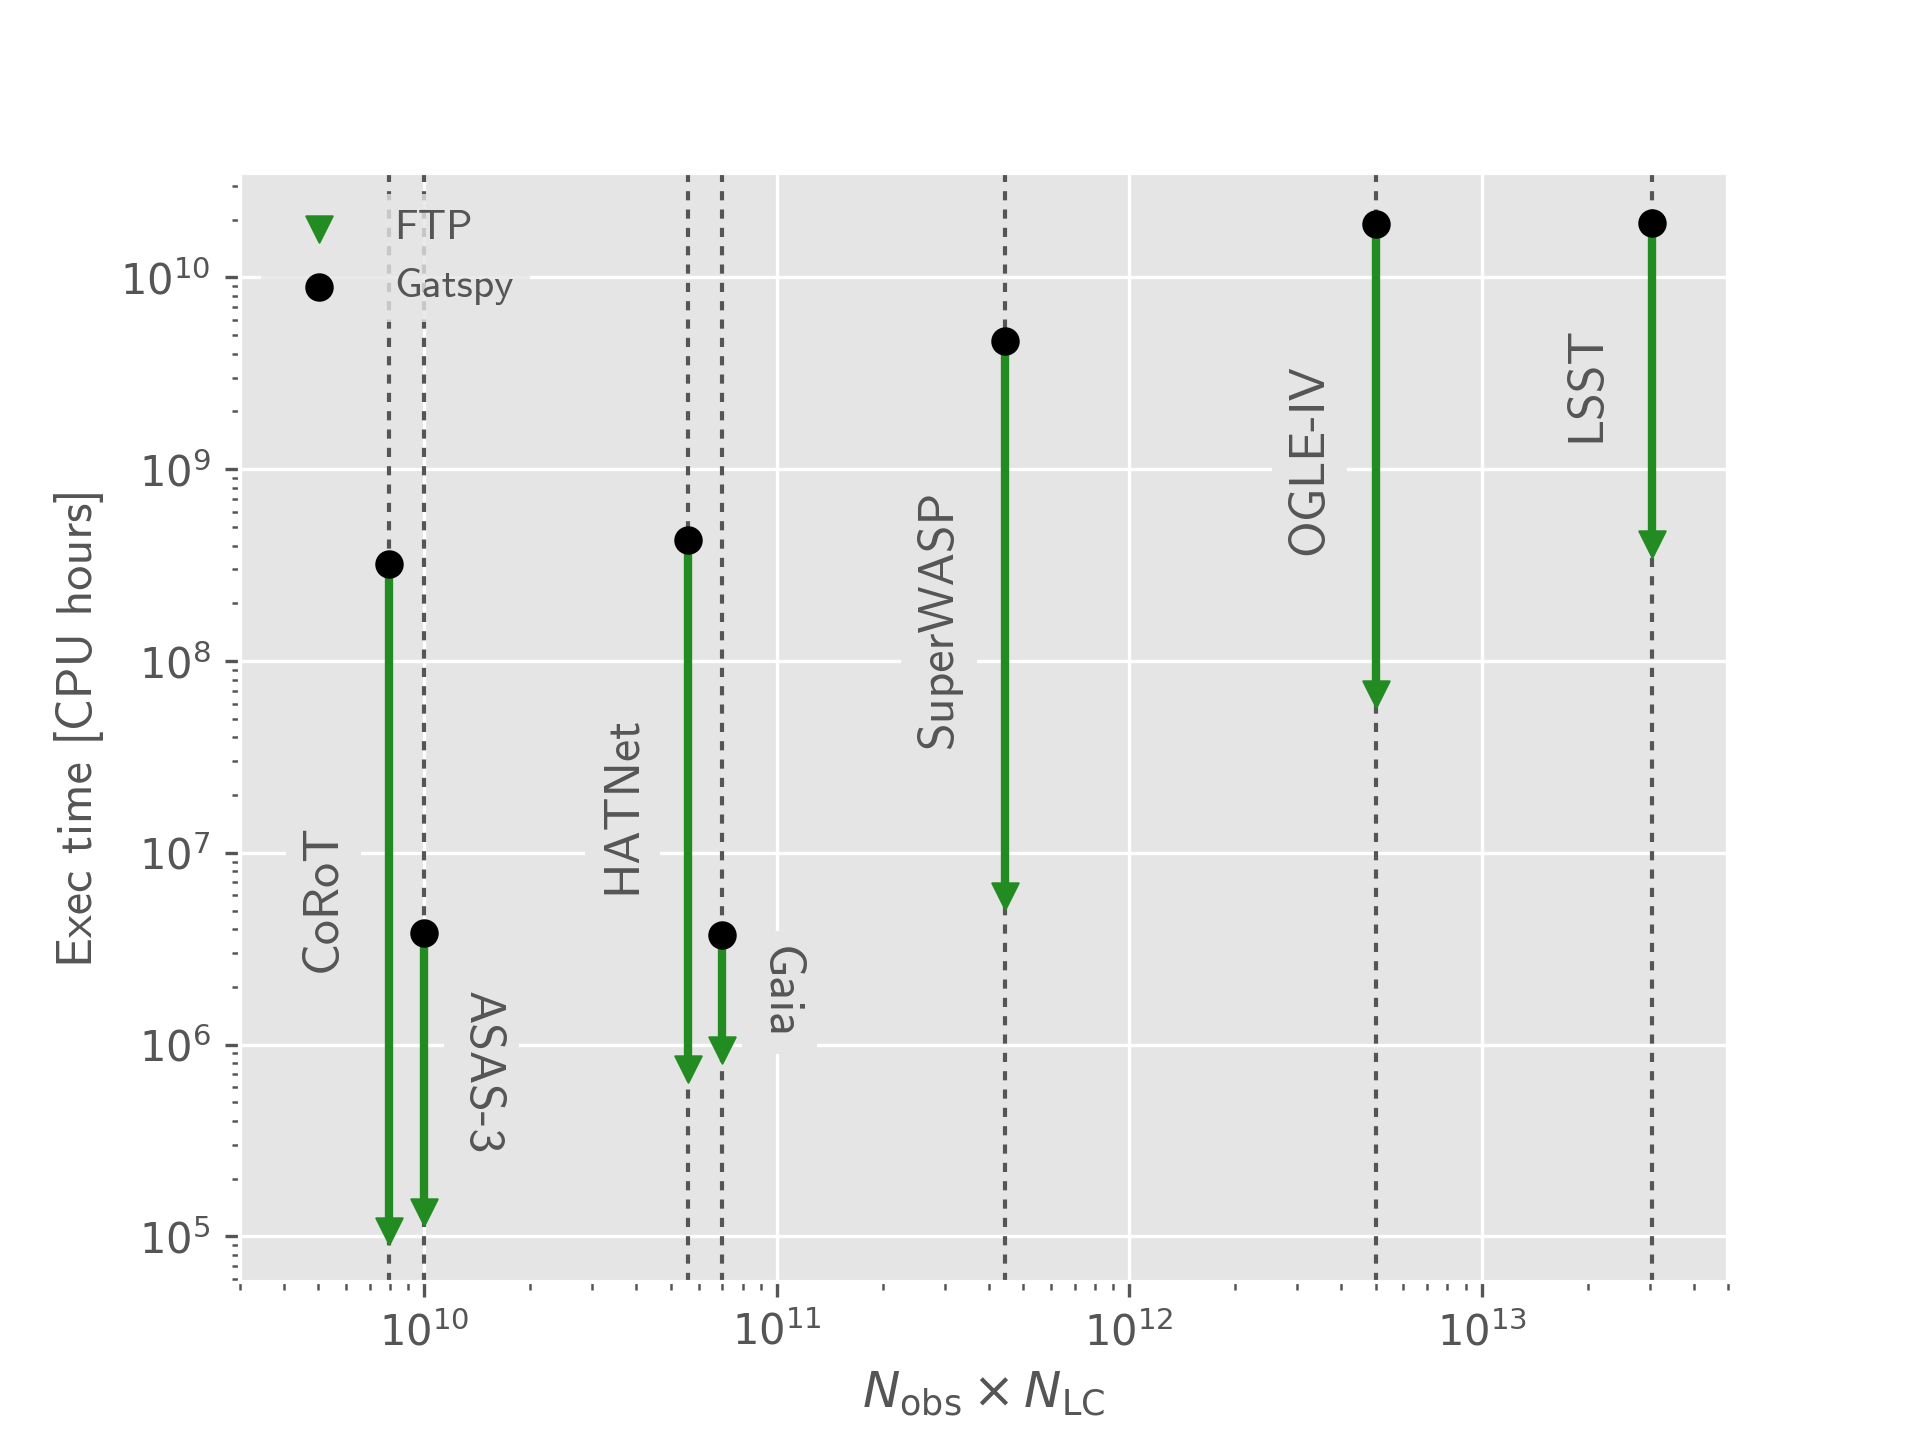
\includegraphics[width=0.5\textwidth]{plots/timing_for_various_surveys.png}
%%\caption{\label{fig:surveys} Computational resources needed for performing 
%a single template periodogram ($H=6$) on an entire survey dataset. Our
%python implementation of FTP improves computational efficiency of template 
%searches by orders of magnitude in most cases, and in one case by over 
%three orders of magnitude (CoRoT). Parameters for $N_{\rm obs}$ and $N_{\rm LC}$
%were estimated from publicly available information (see text).}
%\end{figure}

%As pointed out in \cite{Vanderplas+Ivezic_2015}, current template fitting
%procedures are too slow to be practical for LSST-sized time-domain surveys.
%We attempt to quantify the improvement in computational efficiency for
%several important time-domain surveys, using estimated survey values for 
%$N_{\rm obs}$, the number of observations per object, and $N_{\rm LC}$, 
%the number of objects with lightcurves in the survey. 

%Figure \ref{fig:surveys} shows estimated computation time for a single
%template periodogram performed on the entirety of a given survey. For all
%surveys, the FTP improves computational efficiency in one case over
%three orders of magnitude, but typically between 2-3 orders of magnitude.
%Improving the existing implementation, and porting to C/C++ and CUDA,
%should further improve these numbers.

%Template fitting remains prohibitvely slow for practical applications to
%large time-domain surveys, but this work presents a mathematical shortcut
%that could eventually make template fitting a fast and valuable tool.

%Appendix: Proof that GLS is recovered when H=1
\begin{acknowledgements}
\todo{(acknowledge GRANTS.)}
\end{acknowledgements}
\begin{appendix}
\section{Explicit expression of polynomial condition}

We introduce the following definitions:

\begin{align}
\YMhat &= \savg{y\Mshft}\\
\MMhat &= \savg{\Mshft^2}\\
\Mbar &= \savg{\Mshft}\\
MM &= \MMhat - \Mbar^2\\
YM &= \YMhat - \bar{y}\Mbar
\end{align}

For a given phase shift $\theta_2$, the optimal amplitude and
offset are obtained from requiring the partial derivatives of the
sum of squared residuals, $\chi^2$, to be zero.

Namely, we obtain that
\begin{align}
0 = \frac{\partial\chi^2}{\partial\theta_1} &= 2\sum_iw_i(y_i - \hat{y}_i)\left(-\frac{\partial\hat{y}}{\partial\theta_1}\right)_i\\
    &= \sum_iw_i(y_i - \theta_1\Mshft - \theta_3)\Mshft\\
    &= YM - \theta_1 \MMhat - \theta_3 \Mbar
\end{align}

and
\begin{align}
0 = \frac{\partial\chi^2}{\partial\theta_3} &= 2\sum_iw_i(y_i - \hat{y}_i)\left(-\frac{\partial\hat{y}}{\partial\theta_3}\right)_i\\
    &= \sum_iw_i(y_i - \theta_1\Mshft - \theta_3)\\
    &= \bar{y} - \theta_1 \Mbar - \theta_3
\end{align}

This system of equations can then be rewritten as

\begin{equation}
\begin{pmatrix} \MMhat & \Mbar \\ \Mbar & 1 \end{pmatrix}
\begin{pmatrix} \theta_1 \\ \theta_2 \end{pmatrix}
= 
\begin{pmatrix} \YMhat \\ \bar{y}\end{pmatrix}
\end{equation}

which reduces to 

\begin{equation}
\begin{pmatrix} \theta_1 \\ \theta_2 \end{pmatrix}
= 
\frac{1}{\MMhat - \Mbar^2}
\begin{pmatrix} 1 & -\Mbar \\ -\Mbar & \MMhat \end{pmatrix}
\begin{pmatrix} \YMhat \\ \bar{y}\end{pmatrix}
= 
\frac{1}{\MMhat - \Mbar^2}
\begin{pmatrix} \YMhat - \bar{y}\Mbar \\ \MMhat\bar{y} - \YMhat\Mbar \end{pmatrix}
\end{equation}

Letting $MM = \MMhat - \Mbar^2$ and $YM = \YMhat - \bar{y}\Mbar$, we have
\begin{equation}
\begin{pmatrix} \theta_1 \\ \theta_2 \end{pmatrix}
= 
\begin{pmatrix} YM / MM \\ 1 - \Mbar (YM / MM)\end{pmatrix}
\end{equation}

This means we can rewrite the model $\hat{y} = \theta_1\Mshft + \theta_3$ as 

\begin{equation}
\hat{y}_i = \bar{y} + \left(\frac{YM}{MM}\right)(M_i - \Mbar)
\end{equation}

To obtain an expression for the periodogram, $P = 1 - \chi^2 / \chi^2_0$, we first compute $\chi^2$

\begin{align}
\chi^2 &= \sum_i w_i (y_i - \hat{y}_i)^2 \\
       &= \sum_i w_i (y_i^2 - 2y_i\hat{y}_i + \hat{y}_i^2)\\
       &= \sum_i w_i ((y_i - \bar{y})^2 + 2y_i(\bar{y} - \bar{y} - \left(\frac{YM}{MM}\right)(M_i - \Mbar)) - \bar{y}^2 + \bar{y}^2 \\
       &\qquad + 2\bar{y}\left(\frac{YM}{MM}\right)(M_i - \Mbar) + \left(\frac{YM}{MM}\right)^2(M_i^2 - 2M_i\Mbar + \Mbar^2)\\
       &= YY - 2\frac{(YM)^2}{MM} + \frac{(YM)^2}{MM}\\
       &= YY - \frac{(YM)^2}{MM}
\end{align}

Since, $\chi^2_0 = YY$, we have

\begin{equation}
P(\omega) = \frac{(YM)^2}{YY\cdot MM}
\end{equation}

We wish to maximize $P(\omega)$ with respect to the phase shift parameter $\theta_2$,

\begin{align}
\label{eq:theta2cond}
\partial_{\theta_2}P = 0 &= \frac{YM}{YY\cdot MM}\left(2\partial_{\theta_2}(YM) - \frac{YM}{MM}\partial_{\theta_2}(MM)\right)\\
                         &= 2MM\partial_{\theta_2}(YM) - YM\partial_{\theta_2}(MM).
\end{align}

The final expression is the non-linear condition that must me satisfied by the optimal
phase shift parameter $\theta_2$. However, satisfying Equation \ref{eq:theta2cond}
is not \emph{sufficient} to gaurantee that $\theta_2$ is optimal. The value of the
periodogram at each $\theta_2$ satisfying Equation \ref{eq:theta2cond} must be computed,
and the globally optimal solution chosen from this set.

We seek a more explicit form for Equation \ref{eq:theta2cond}. We first
derive expressions for $MM$ and $YM$.

\begin{align}
MM &\equiv \sum_i w_i M_i^2\\
   &= \sum_i w_i \left(\sum_nA_n\cos{\omega n t_i} + B_n\sin{\omega n t_i}\right)^2\\
   &= \sum_n \sum_m A_nA_mCC_{nm} + (A_nB_mCS_{nm} + B_nA_m(CS^T)_{nm}) + B_nB_mSS_{nm}\\
   &= \sum_n \sum_m A_nA_mCC_{nm} + 2A_nB_mCS_{nm} + B_nB_mSS_{nm}\\
\end{align}


Recall that

\begin{align}
A_n(x) &= c_n T_n(x) - s_nq\sqrt{1-x^2}U_{n-1}(x)\\
B_n(x) &= s_n T_n(x) + c_nq\sqrt{1-x^2}U_{n-1}(x)\\
\end{align}

The expressions for $A_n(x)$ and $B_n(x)$ can be rewritten as

\begin{align}
A_n(x) &= c_nT_n(x) - qs_n\sqrt{1-x^2}U_{n-1}(x)\\
       &= \left(\frac{c_n - iqs_n}{2}\right)\left(T_n(x) + \sqrt{x^2 - 1}U_{n-1}(x)\right) + \\
       &\quad \left(\frac{c_n + iqs_n}{2}\right)\left(T_n(x) - \sqrt{x^2 - 1}U_{n-1}(x)\right)\\
B_n(x) &=  \left(\frac{s_n + iqc_n}{2}\right)\left(T_n(x) + \sqrt{x^2 - 1}U_{n-1}(x)\right) + \\
       &\quad \left(\frac{s_n - iqc_n}{2}\right)\left(T_n(x) - \sqrt{x^2 - 1}U_{n-1}(x)\right)
\end{align}

The Chebyshev polynomials satisfy the following property:

\begin{equation}
T_n(x) + \sqrt{x^2 - 1}U_{n-1}(x) = (x + \sqrt{x^2 - 1})^n
\end{equation}

From which we can also derive that

\begin{equation}
T_n(x) - \sqrt{x^2 - 1}U_{n-1}(x) = (x + \sqrt{x^2 - 1})^{-n}.
\end{equation}

This provides a convenient change of variables

\begin{equation}
y = x + \sqrt{x^2 - 1}
\end{equation}

with which to rewrite $A_n$ and $B_n$
\begin{align}
A_n(y) &= \left(\frac{c_n - iqs_n}{2}\right)y^n + \left(\frac{c_n + iqs_n}{2}\right)y^{-n}\\
       &= \alpha_ny^n + \alpha^{*}_ny^{-n}\\
B_n(y) &= \left(\frac{s_n + iqc_n}{2}\right)y^n + \left(\frac{s_n - iqc_n}{2}\right)y^{-n}\\
       &= (iq)\left(\alpha_ny^n - \alpha^{*}_ny^{-n}\right)\\
A_nA_m &= \left(\alpha_ny^n + \alpha^{*}_ny^{-n}\right)\left(\alpha_my^m + \alpha^{*}_my^{-m}\right)\\
       &= \alpha_n\alpha_m y^{n+m} + \alpha^{*}_n\alpha_my^{m-n} + \alpha_n\alpha^{*}_m y^{n-m} + \alpha^{*}_n\alpha^{*}_my^{-(n+m)}\\
A_nB_m &= (iq)\left(\alpha_ny^n + \alpha^{*}_ny^{-n}\right)\left(\alpha_my^m - \alpha^{*}_my^{-m}\right)\\
       &= (iq)\left\{\alpha_n\alpha_m y^{n+m} + \alpha^{*}_n\alpha_my^{m-n} - \alpha_n\alpha^{*}_m y^{n-m} - \alpha^{*}_n\alpha^{*}_my^{-(n+m)}\right\}\\
B_nB_m &= -\left(\alpha_ny^n - \alpha^{*}_ny^{-n}\right)\left(\alpha_my^m - \alpha^{*}_my^{-m}\right)\\
       &= -\left\{\alpha_n\alpha_m y^{n+m} - \alpha^{*}_n\alpha_my^{m-n} - \alpha_n\alpha^{*}_m y^{n-m} + \alpha^{*}_n\alpha^{*}_my^{-(n+m)}\right\}
\end{align}

Now we have that 

\begin{align}
MM_{nm} &= A_nA_mCC_{nm} + 2A_nB_mCS_{nm} + B_nB_mSS_{nm}\\
        &= \alpha_n\alpha_m\left(CC_{nm} + 2(iq)CS_{nm} - SS_{nm}\right)y^{n+m}\\
        &\quad + 2\alpha_n\alpha^{*}_m\left(CC_{nm} - \frac{iq}{2}\left(CS_{nm} - CS^{T}_{nm}\right) - SS_{nm}\right)y^{n-m}\\
        &\quad + (\alpha_n\alpha_m)^{*}\left(CC_{nm}  - 2(iq)CS_{nm} + SS_{nm}\right)y^{-(n+m)}\\
        &= \alpha_n\alpha_m\CCt_{nm}y^{n+m} + 2\alpha_n\alpha^{*}_m\CSt_{nm}y^{n-m} + \alpha^{*}_n\alpha^{*}_m\SSt_{nm}y^{-(n+m)}
\end{align}

and for $YM$:

\begin{align}
YM_{k} &= A_kYC_k + B_kYS_k\\
        &= \alpha_kYC_ky^k + \alpha_k^{*}YC_ky^{-k} + (iq)\left(\alpha_kYS_ky^k - \alpha^{*}_kYS_ky^{-k}\right)\\
        &= (YC_k + iqYS_k)\alpha_ky^k + (YC_k - iqYS_k)\alpha^{*}_ky^{-k}\\
        &= \alpha_k\YCt_k y^k + \alpha^{*}_k\YCt_k^{*} y^{-k}
\end{align}

since $n,m,k > 0$, we also have that

\begin{align}
\partial YM_k &= k\left(\alpha_k\YCt_k y^{k-1} - \alpha^{*}_k\YCt_k^{*} y^{-(k+1)}\right)\\
\partial MM_{nm} &= (n+m)\alpha_n\alpha_m\CCt_{nm}y^{n+m-1} + 2(n-m)\alpha_n\alpha^{*}_m\CSt_{nm}y^{n-m-1} \\
                &\quad- (n+m)\alpha^{*}_n\alpha^{*}_m\SSt_{nm}y^{-(n+m+1)}
\end{align}

and thus the final polynomial expression for $y$ can be derived by expanding Equation \ref{eq:theta2cond} in terms of $y$ and multiplying through by
 $y^{3H+1}$, to eliminate any polynomial terms in $(1/y)$.

\begin{align}
2k&\left(\alpha_k\YCt_k y^{H+k} - \alpha^{*}_k\YCt_k^{*} y^{H-k}\right)\left(\alpha_n\alpha_m\CCt_{nm}y^{2H+n+m} \right.\\
&\qquad\qquad\left. + 2\alpha_n\alpha^{*}_m\CSt_{nm}y^{2H + n - m} + \alpha^{*}_n\alpha^{*}_m\SSt_{nm}y^{2H-n-m)}\right)\\
& - \left(\alpha_k\YCt_k y^{H+k} + \alpha^{*}_k\YCt_k^{*} y^{H-k}\right)\left((n+m)\alpha_n\alpha_m\CCt_{nm}y^{2H+n+m} \right.\\
&\qquad\qquad\left. + 2(n-m)\alpha_n\alpha^{*}_m\CSt_{nm}y^{2H+n-m} - (n+m)\alpha^{*}_n\alpha^{*}_m\SSt_{nm}y^{2H-n-m}\right) = 0
\end{align}

This could be expanded, however, it is usually more computationally efficient to compute four separate polynomials (that scale as $\bigO(H^2)$ and $\bigO(H)$),
and performing two polynomial multiplication operations, which allow for the use of fast polynomial libraries.


\end{appendix}
\bibliographystyle{apj}
\bibliography{refs}
\end{document}
